\documentclass[border=10pt]{standalone}
\usepackage{pgfplots}
\pgfplotsset{compat=1.18}
\begin{document}
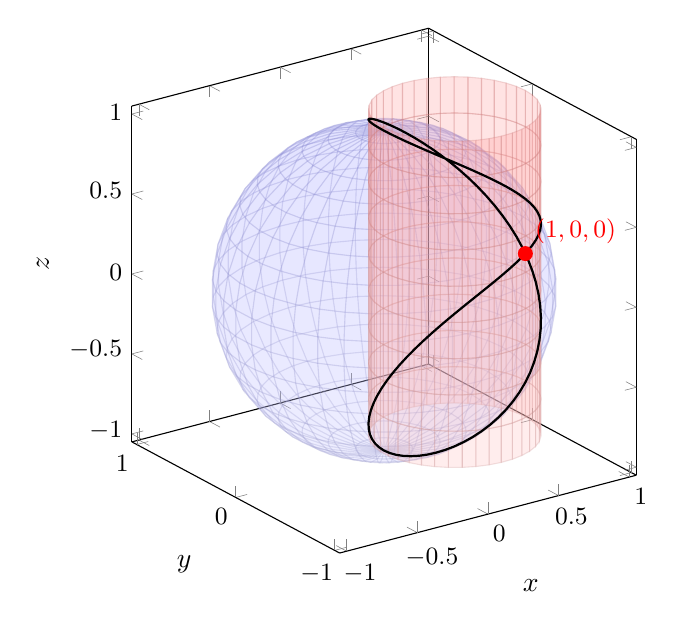
\begin{tikzpicture}
\begin{axis}[
    view={-35}{22},
    unit vector ratio=1 1 1,
    xmin=-1.05, xmax=1.05,
    ymin=-1.05, ymax=1.05,
    zmin=-1.05, zmax=1.05,
    xlabel=$x$, ylabel=$y$, zlabel=$z$,
    tick label style={font=\small},
    width=10cm, height=9cm,
]
% Sphere of radius 1, light blue
\addplot3[
    surf,
    opacity=0.18,
    domain=0:180,
    y domain=0:360,
    samples=20,
    samples y=40,
    colormap={myblue}{color=(blue!20) color=(blue!35)},
]
({sin(x)*cos(y)}, {sin(x)*sin(y)}, {cos(x)});

% Cylinder r = cos(theta), light red
\addplot3[
    surf,
    opacity=0.28,
    domain=0:360,
    y domain=-1.02:1.02,
    samples=40,
    samples y=10,
    colormap={myred}{color=(red!25) color=(red!40)},
]
({0.5+0.5*cos(x)}, {0.5*sin(x)}, {y});

% Intersection curves
\addplot3[thick, black, domain=-90:90, samples=60]
    ({cos(x)^2}, {cos(x)*sin(x)}, {abs(sin(x))});
\addplot3[thick, black, dashed, domain=-90:90, samples=60]
    ({cos(x)^2}, {cos(x)*sin(x)}, {-abs(sin(x))});

% Point (1,0,0)
\addplot3[only marks, mark=*, mark size=2.5pt, color=red] coordinates {(1,0,0)};
\node[anchor=south west, font=\small, color=red] at (axis cs:1,0,0) {$(1,0,0)$};
\end{axis}
\end{tikzpicture}
\end{document}
